\documentclass[UTF8,a4paper,twoside]{ctexart}

% 封面信息
\newcommand{\stuname}{王五}			 	  % 学生姓名
\newcommand{\stuid}{3150000000}		  		 % 学生学号
\newcommand{\teaname}{李四}		    	  % 指导教师
\newcommand{\stugrade}{15级}			 		% 学生年级
\newcommand{\stumajor}{电子信息工程} 	 		% 学生专业
\newcommand{\stucollege}{电气工程学院} 		% 学生所在学院
\newcommand{\stutitle}{毕业设计题目}			% 毕设题目

% 页面设置
% A4纸张大小 上下左边边距参考Word中"适中"类型
% A4纸张宽21cm 高29.7cm
\usepackage{geometry}	
\geometry{left=1.91cm, right=1.91cm, top=2.54cm, bottom=2.54cm}
% 设置首行缩进2字符
% 使用 \noindent 命令可以取消缩进
\usepackage{indentfirst}
\setlength{\parindent}{2em}

% 字体设置
\usepackage{fontspec}
% 在cmd中输入fc-list :lang=en >> d:\font.txt可以获取电脑中所有英文字体
% 在cmd中输入fc-list :lang=zh >> d:\font.txt可以获取电脑中所有中文字体
\setmainfont{Times New Roman}						% 缺省英文字体为Times New Roman
\setCJKmainfont[BoldFont=SimHei]{FangSong}			% 缺省中文字体为 仿宋
% 粗体为中文字体 黑体
\setCJKfamilyfont{fs}{FangSong}
\newcommand{\zhengwen}{\CJKfamily{fs}\zihao{-4}}	% 正文字体 仿宋小4号
\setCJKfamilyfont{STfs}{STFangsong}
\newcommand{\cover}{\CJKfamily{STfs}\zihao{3}}
\setCJKfamilyfont{song}{SimSun}
\newcommand{\header}{\CJKfamily{song}\zihao{-5}}
\newcommand{\imageortable}{\CJKfamily{song}\zihao{5}\bfseries}

% 行距设置
\usepackage{setspace}
\linespread{1.5}\selectfont		% 1.5倍字号,这与word中的1.5倍行距有一点差别

% 多级标题设置
\usepackage{titlesec}
\setcounter{secnumdepth}{4}		% 设置标题层次共4层
\titleformat{\section}[block]{\centering\zihao{3}\bfseries}{\chinese{section}、}{0pt}{}
\titleformat{\subsection}[block]{\zihao{-3}\bfseries}{\arabic{subsection}}{0.5em}{}
\titleformat{\subsubsection}[block]{\zihao{4}\bfseries}{\arabic{subsection}.\arabic{subsubsection}}{0.5em}{}
\titleformat{\paragraph}{\zihao{4}\bfseries}{\arabic{subsection}.\arabic{subsubsection}.\arabic{paragraph}}{0.5em}{}
% 设置段间距
\titlespacing{\section}{0pt}{12pt}{6pt}				% 标题1 段前12磅 段后6磅
\titlespacing{\subsection}{0pt}{13pt}{13pt}			% 标题2 段前13磅 段后13磅
\titlespacing{\subsubsection}{0pt}{13pt}{13pt}		% 标题3 段前13磅 段后13磅
\titlespacing{\paragraph}{0pt}{13pt}{13pt}			% 标题4 段前13磅 段后13磅

% 插入图片宏包
% 多个浮动体连续排布用参数H进行固定,如下所示,不用H会出现难以预料的排布
% \begin{figure}[H]
% content...
% \end{figure}
\usepackage{graphicx}
\usepackage{subfigure}
\usepackage{caption}
\usepackage{float}
\captionsetup{labelsep=quad,labelfont=bf,font=singlespacing}
\renewcommand{\thefigure}{\arabic{section}.\arabic{figure}}

% 插入表格宏包
\usepackage{booktabs}
\usepackage{longtable}
\usepackage{multirow}
\usepackage{array}
\renewcommand{\thetable}{\arabic{section}.\arabic{table}}
\usepackage{enumerate}

% 设置目录
\usepackage{titletoc}
\setcounter{tocdepth}{4}
\renewcommand{\thesection}{\chinese{section}、}
\renewcommand{\thesubsection}{\arabic{subsection}}
\renewcommand{\thesubsubsection}{\arabic{subsection}.\arabic{subsubsection}}
\renewcommand{\theparagraph}{\arabic{subsection}.\arabic{subsubsection}.\arabic{paragraph}}
\titlecontents{section}[2em]{\bfseries\zihao{-4}}{\contentslabel{2em}}{}{\titlerule*[0.5pc]{$\cdot$}\contentspage}
\titlecontents{subsection}[2.5em]{\bfseries\zihao{-4}}{\contentslabel{1em}}{}{\titlerule*[0.5pc]{$\cdot$}\contentspage}
\titlecontents{subsubsection}[4.5em]{\zihao{-4}}{\contentslabel{1.83em}}{}{\titlerule*[0.5pc]{$\cdot$}\contentspage}
\titlecontents{paragraph}[5.5em]{\zihao{-4}}{\contentslabel{2.67em}}{}{\titlerule*[0.5pc]{$\cdot$}\contentspage}
% 超链接
% colorlinks=true 超链接以颜色表示 false 超链接以方框框出
% linkcolor 指定颜色
% CJKbookmarks 让链接支持中文
\usepackage[colorlinks=true,linkcolor=black,citecolor=black,CJKbookmarks=true]{hyperref}
\newcommand{\myeqref}[1]{式 (\ref{#1})}
\newcommand{\mytaref}[1]{表 \ref{#1}}
\newcommand{\myfiref}[1]{图 \ref{#1}}

% 设置页眉页脚
\usepackage{fancyhdr}
\pagestyle{fancy}
\fancypagestyle{Index}{
	\setcounter{page}{1}\pagenumbering{Roman}
	\fancyhead[L]{}
	\fancyhead[R]{\header \stutitle}
}
\fancypagestyle{Content}{
	\setcounter{page}{1}\pagenumbering{arabic}
	\fancyhead[LO]{}
	\fancyhead[RO]{\header \stutitle}
	\fancyhead[LE]{\header 浙江大学本科生毕业论文}
	\fancyhead[RE]{}
	\fancyfoot[C]{\zihao{-5} \thepage}
}

% 设置参考文献
\usepackage{natbib}

% 插入公式
\usepackage{amsmath}
\usepackage{indentfirst}


\begin{document}
	
	% 封面
	\begin{center}
	\vspace*{1ex}
	
\includegraphics[width=11cm]{images/zju.jpg} 
		
	\vspace{1ex}
	\zihao{-1}\bfseries
	本\ \ 科\ \ 生\ \ 毕\ \ 业\ \ 设\ \ 计(论\ \ 文)
		
	\vspace{1ex}
	文献综述和开题报告
		
	\vspace{3ex}
	
\includegraphics[width=3.5cm]{images/qsy.jpg}
	
	\cover	
	\vspace{5ex}
	\makebox[3.2cm][l]{姓名与学号}\underline{\makebox[7cm]{王秦松\qquad 3150102980}}
	
	\vspace{2ex}
	\makebox[3.2cm][l]{指导教师}\underline{\makebox[7cm]{王xx}}
	
	\vspace{2ex}
	\makebox[3.2cm][l]{年级与专业}\underline{\makebox[7cm]{15级电子信息工程}}
	
	\vspace{2ex}
	\makebox[3.2cm][l]{所在学院}\underline{\makebox[7cm]{电气工程学院}}
\end{center}


	
	% 目录
	\newpage
	\pagestyle{Index}
	\tableofcontents
	
	% 正文
	\newpage
	\pagestyle{Content}\zhengwen
\section{文献综述}
	 	
\subsection{背景介绍}
这是\LaTeX。
		
\noindent 测试测试
	
\subsubsection{公式}
公式见\myeqref{eq:1}
\begin{equation}
\label{eq:1}
a^2 + b^2 = c^2
\end{equation}
	
\paragraph{图片}

图片见\myfiref{Wallpaper}

\vspace{10ex}
\begin{figure}[H]
	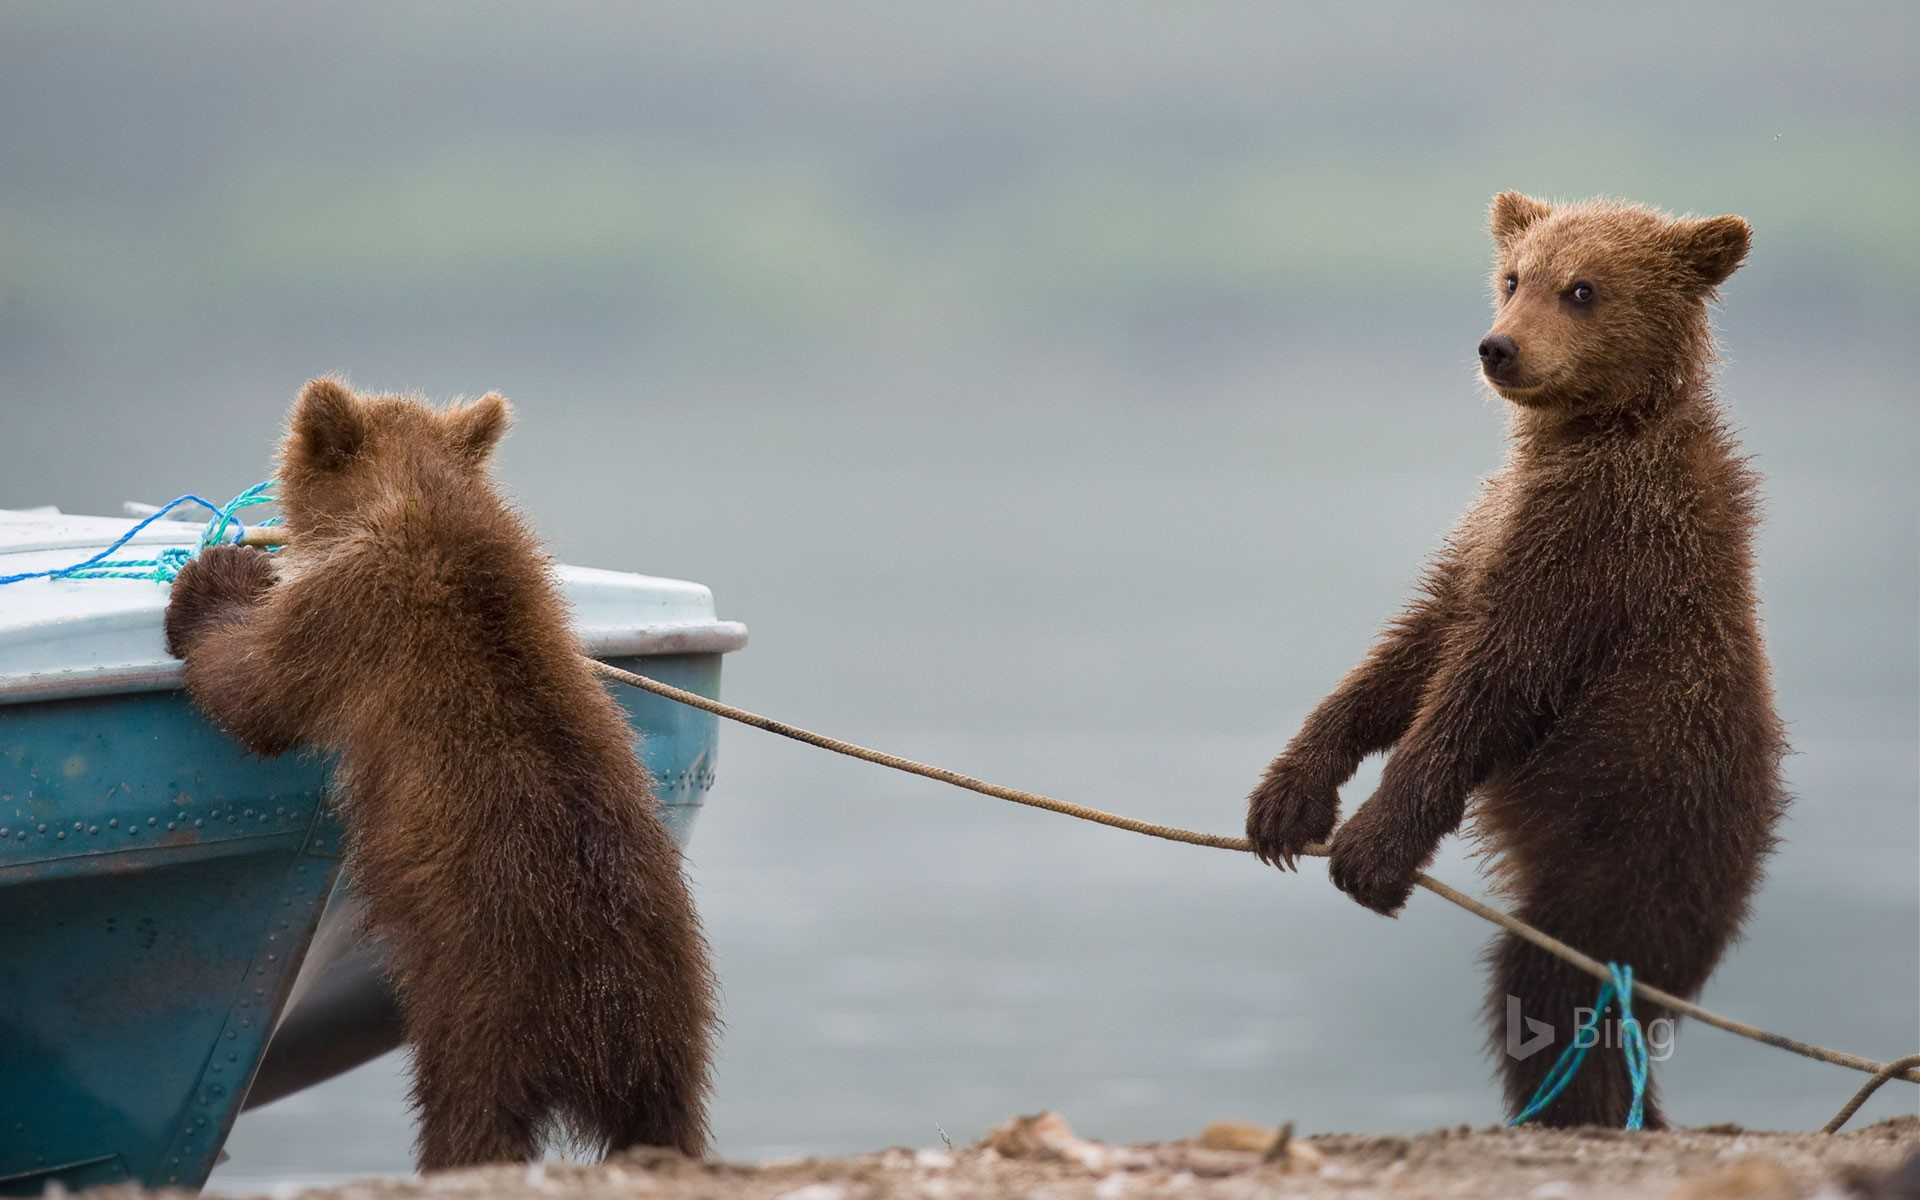
\includegraphics[width=\textwidth]{images/BingWallpaper-2019-04-01.jpg}
	\caption{第一张图}\label{Wallpaper}
\end{figure}
	
\subsection{国内外研究现状}
	
\subsubsection{研究方向及进展}
	
\subsubsection{存在问题}
	
\subsection{研究展望}
	\section{开题报告}

\subsection{问题提出的背景}

\subsubsection{背景介绍}
引用\cite{schweizer2013comparative}

\paragraph{段的标题}

\subsubsection{本研究的意义和目的}

\subsection{论文的主要内容和技术路线}

\subsubsection{主要研究内容}

\subsubsection{技术路线}

\subsubsection{可行性分析}

\subsection{研究计划进度安排及预期目标}

\subsubsection{进度安排}

\subsubsection{预期目标}
	\section{外文翻译}

	\section{外文原文}
	
	% 参考文献
	\newpage
	\bibliographystyle{unsrt}
	\phantomsection		% 要想目录中参考文献的超链接正确需要加这一语句
	\addcontentsline{toc}{section}{参考文献}
	\bibliography{reference/refs}
			
\end{document}